\chapter{Evaluation of Mashup Composers}
\label{chapter:evaluation}

This chapter deals with the evaluation of existing tools, which are used for composing and
designing mashups. First, the most important features of each tool are discussed before the tools
are evaluated against certain evaluation criteria. These criteria represent requirements for realizing the air
ambulance scenario (see Section \ref{sec:scenario}) or similar ones.

The evaluation process is based on \cite{Heinrich2000} and therefore starts with the evaluation
preparation.

\section{Evaluation Preparation}

The evaluation preparation section introduces the various evaluation objects
and defines the goals and criteria for the evaluation process.

\subsection{Evaluation Objects}
\label{sec:evaluation_objects}

The inspected evaluation objects are different software products for designing mashup components
without the need for writing any code. To select respective products an extensive search was
conducted to find information on mashups and mashup-composers. This search resulted in a list of
ten to fifteen tools which were shortlisted and from which Microsoft Popfly, Yahoo Pipes and IBM Mashup
Center were selected. These three tools are not only the most popular ones, but also the most
advanced. All of them are - at least as test version - available to the public. The fact that
big companies like Microsoft, Yahoo and IBM stand behind these tools provides further arguments for
the choice.

In the following the selected tools are introduced.

\subsubsection{Microsoft Popfly}
\label{sec:microsoft_popfly}

As stated on the official Popfly Website \cite{microsoft_popfly},

\msQuote{Microsoft Popfly is the fun, easy way to build and share mashups,
gadgets, games, web pages, and applications. Popfly consists of a set of online
visual tools for building web pages and mashups, and a social network of creators
where you can host, share, rate, comment and even remix creations from other
Popfly users.}

\par This statement shows that Microsoft Popfly is not only designed to create simple mashups, but also to set up web pages and games. Nevertheless, the main
focus of this work will lie on the mashup-feature of this tool.

Therefore, the next section introduces the ``Mashup Creator'', which provides an
interface for composing mashups. Figure
\ref{fig:microsoft_popfly_tool_architecture} gives an overview of the mashup structure and the
involved software products that are needed to compose mashups with Microsoft Popfly.

\begin{figure}
	\centering
	\fbox{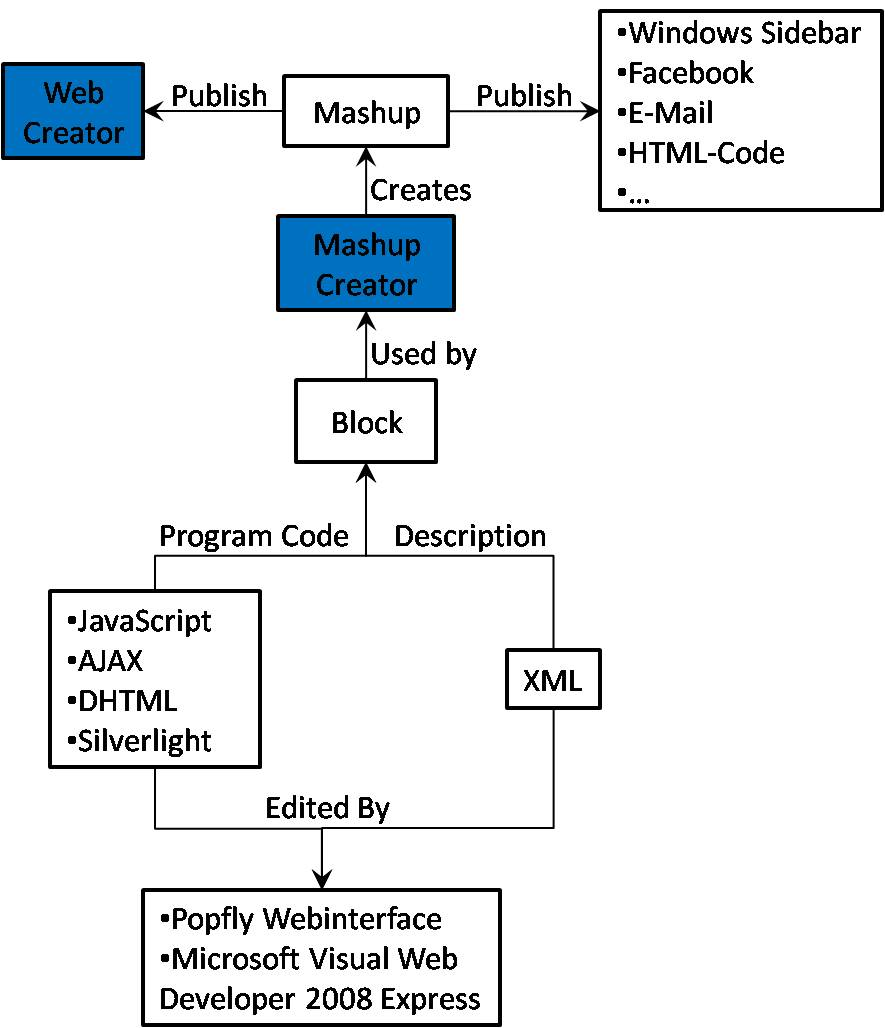
\includegraphics[width=0.8\textwidth]{Bilder/microsoft_popfly_tool_architecture.jpg}}
	\caption{Microsoft Popfly - Overview}
	\label{fig:microsoft_popfly_tool_architecture}
\end{figure}

\paragraph{Mashup Creator}

The Mashup Creator, like all other Popfly tools, is provided as web application and can therefore
be accessed via the Popfly website.

\begin{figure}
	\centering
	\fbox{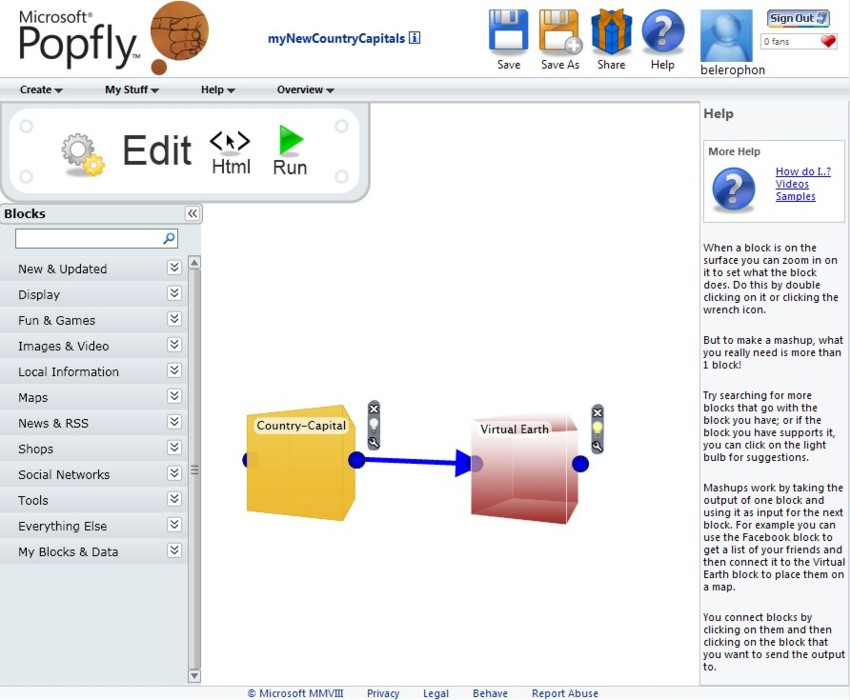
\includegraphics{Bilder/microsoft_popfly_mashup_creator.jpg}}
	\caption{Microsoft Popfly - Mashup Creator}
	\label{fig:microsoft_popfly_mashup_creator}
\end{figure}

To compose mashups, the tool provides a simple user interface with a working
area and a catalog of basic building units, which are called ``blocks''. These blocks consist of
two parts: One part contains the program code, which implements the functionality, the other one is an
XML-Metadata file, which describes the block and its functionality in a human readable form.

The program code of simple data access blocks is written in
JavaScript\footnote{JavaScript is an object-oriented scripting language, which
allows the development of enhanced user interfaces and websites.}, whereas more
complex presentation layer blocks like ``Virtual Earth'' are based on
AJAX\footnote{asynchronous JavaScript and XML}, DHTML\footnote{DHTML is a
collection of technologies like HTML and JavaScript used together.} or
Silverlight.

In order to extend the already large catalog of pre-built blocks and to enable
the building of new blocks or editing existing ones, Microsoft provides a simple
web-interface to edit the JavaScript code. In addition, Microsoft provides the ``Popfly
Explorer''-plug-in for the freely available ``Microsoft Visual Web Developer 2008 Express'' as an
alternative to create and edit more complex blocks.

The pre-built blocks are sufficient for creating simple mashups without having to implement custom
blocks.

Figure \ref{fig:microsoft_popfly_mashup_creator} shows the Mashup Composer with two interconnected
blocks.

\paragraph{Using the created Mashup}
As soon as the mashup creation process is finished the mashup can be saved, published to other
Popfly users, to the Windows sidebar, to a Facebook profile or to various other social networking sites and
integrated into websites. The integration into websites is also supported by the so-called ``Web
Creator'', which is a part of Microsoft Popfly and is used to design simple websites.

\paragraph{The concept of a Mashup within Microsoft Popfly}
Each Microsoft Popfly mashup comprises the following parts (remember the
structure of a mashup described in Section \ref{sec:mashup}):

\begin{enumerate}
\item Every mashup needs one or more of the various \textbf{data source}
blocks. This can be the Flickr photo database, some RSS-feed, a database of the
capitals of all countries, as well as many other kinds of data sources.\newline
Furthermore, Popfly provides blocks for user inputs, which enable, for example,
the specification of RSS-feed URLs at runtime.

\item The second essential part of a mashup is the \textbf{display}, which
presents the information, received from the data source blocks, in a suitable
form. Therefore, Popfly provides blocks like virtual earth, image slide-show
displays or simple tables with a few columns.

\item The third major part is the ability to \textbf{connect two blocks} in order
to exchange data and communicate respectively.\newline Naturally, most blocks
offer not only a single function that can be called and there can be
compatibility problems concerning the data that is transferred between the
blocks. Therefore, most blocks have to be edited slightly or additional blocks,
which convert and process the data, have to be introduced.\newline In the case of
Virtual Earth (see Figure \ref{fig:microsoft_popfly_edit_block}) the operation,
which processes the data of the data source block, can be chosen,
input-parameters for this operation can be specified and additional properties
can be defined (see Figure
\ref{fig:microsoft_popfly_concept_of_a_block}). As the Virtual Earth
block in the depicted example gets its data from the Country-Capital block, this
block is enabled as data source. If there is no compatible data source block
available, the input fields can be filled with custom values.
\end{enumerate}

\begin{figure}
	\centering
		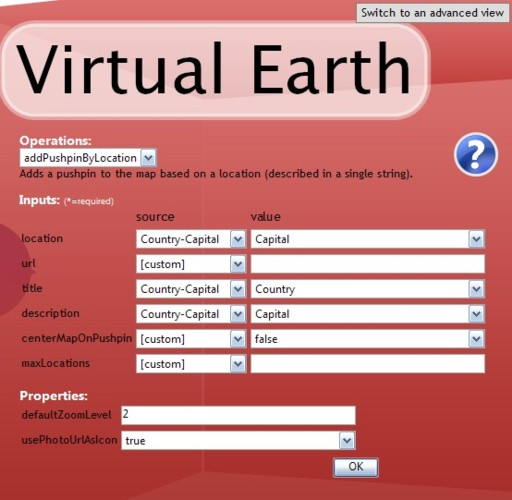
\includegraphics{Bilder/microsoft_popfly_edit_block.jpg}
	\caption{Microsoft Popfly - Editing the Virtual Earth block}
	\label{fig:microsoft_popfly_edit_block}
\end{figure}

\begin{figure}
	\centering
	\fbox{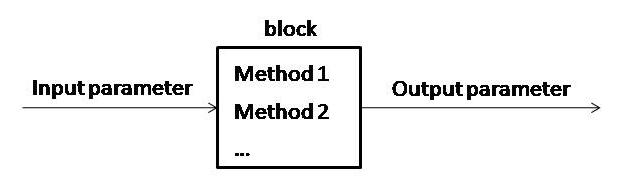
\includegraphics[width=0.8\textwidth]{Bilder/microsoft_popfly_block.jpg}}
	\caption{Microsoft Popfly - Structure of a block}
	\label{fig:microsoft_popfly_concept_of_a_block}
\end{figure}

The mashup depicted in Figure \ref{fig:microsoft_popfly_capitals} is one of the simplest mashups that
can be created and is based on the structure which is depicted in Figure
\ref{fig:microsoft_popfly_concept_of_a_simple_mashup}. Naturally most mashups do not only consist of
two building blocks, but are more complex. Therefore, Microsoft provides, for example, blocks to
combine or merge two or more data sources, to filter special data and to check if the data complies
with certain conditions to support various different application scenarios. For better
understandability Figure \ref{fig:microsoft_popfly_concept_of_a_complex_mashup} depicts the
structure of such a complex mashup.

\begin{figure}
	\centering
		\fbox{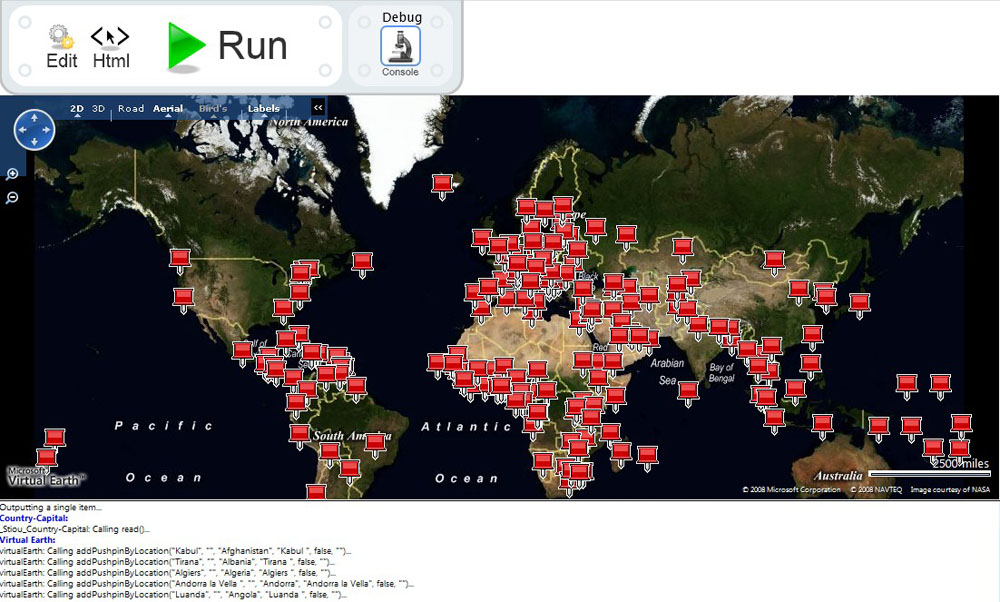
\includegraphics[width=0.8\textwidth]{Bilder/microsoft_popfly_capitals.jpg}}
	\caption{Microsoft Popfly - The ``Country Capitals'' Mashup in Action}
	\label{fig:microsoft_popfly_capitals}
\end{figure}

\begin{figure}
	\centering
	\fbox{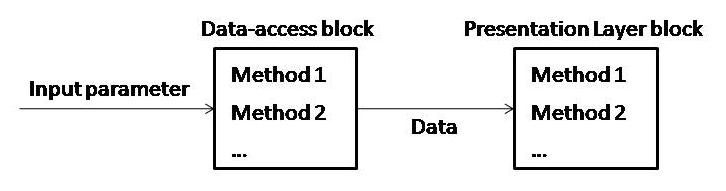
\includegraphics[width=0.8\textwidth]{Bilder/microsoft_popfly_simple_mashup.jpg}}
	\caption{Microsoft Popfly - Structure of a simple Mashup}
	\label{fig:microsoft_popfly_concept_of_a_simple_mashup}
\end{figure}

\begin{figure}
	\centering
	\fbox{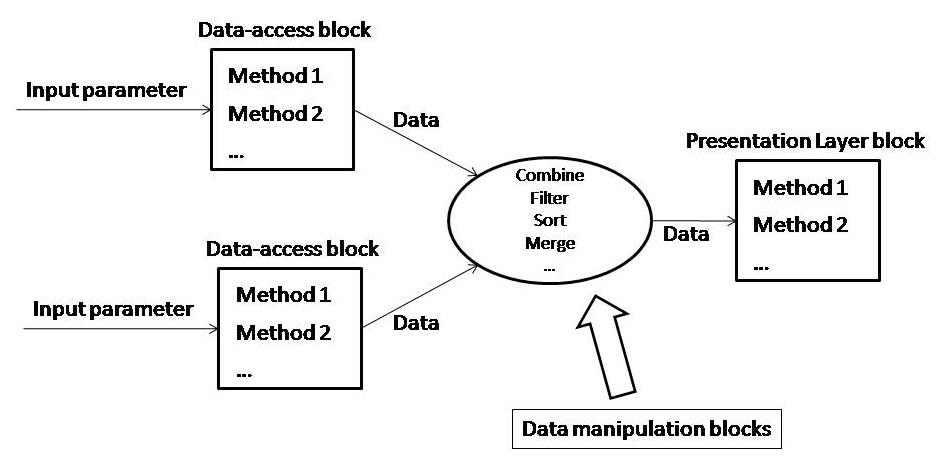
\includegraphics[width=0.8\textwidth]{Bilder/microsoft_popfly_complex_mashup.jpg}}
	\caption{Microsoft Popfly - Structure of a complex Mashup}
	\label{fig:microsoft_popfly_concept_of_a_complex_mashup}
\end{figure}

\paragraph{Mashup Execution}
To test and use the created mashup, Microsoft Popfly differentiates between build and execution
time. This means that the output of the composed mashup is only displayed when it is executed by
``running'' the mashup as it is called. The resulting mashup (see Figure
\ref{fig:microsoft_popfly_capitals}) is loaded within the Mashup Creator and a debug console can be
displayed to analyze possible errors. Switching between ``edit'' and ``run'' mode can be done
easily and hence allows a quick and smooth adaptation of the built mashup.

\subsubsection{Yahoo Pipes}
\label{sec:yahoo_pipes}

The second tool that is analyzed and tested is also a web application, is
developed by Yahoo and called ``Yahoo Pipes'' \cite{yahoo_pipes}. It allows the
creation and modification of pipes, as mashups are called within Yahoo Pipes, as
well as browsing through pipes designed by other individuals.

\paragraph{The Pipes Editor}
Similar to Microsoft Popfly, the pipes editor (see Figure
\ref{fig:yahoo_pipes_pipes_editor}) provides a list of building blocks which are
called ``modules'' and a working area. Important to mention here is that the
catalog of building blocks can not be extended, but the development team has to be contacted and
informed about missing features instead.

\begin{figure}
	\centering
		\fbox{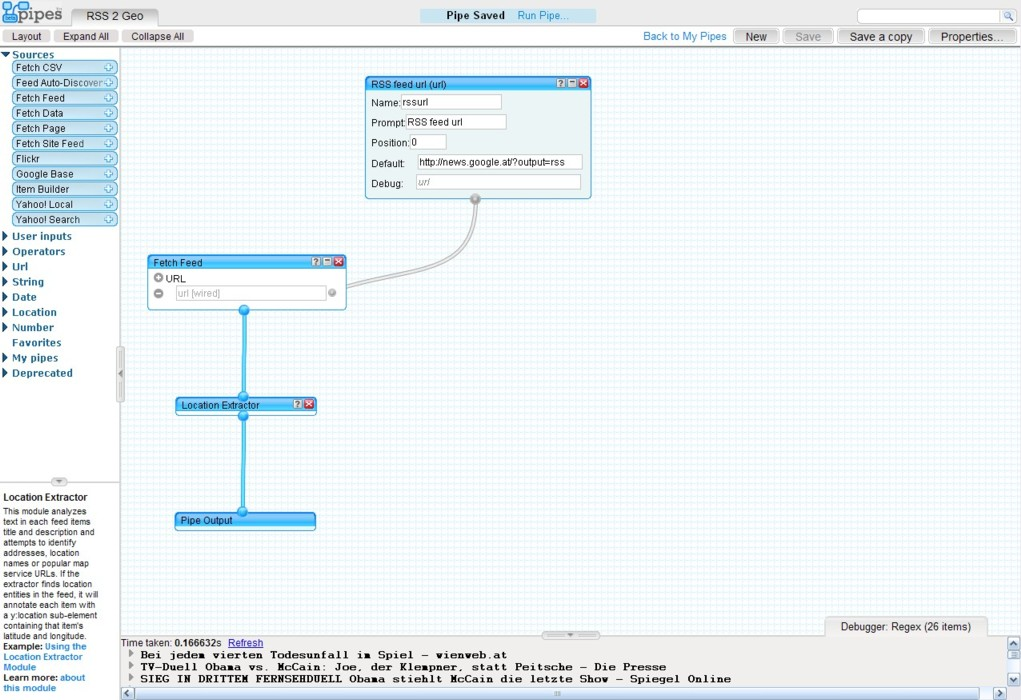
\includegraphics{Bilder/yahoo_pipes_pipes_editor.jpg}}
	\caption{Yahoo Pipes - The Pipes Editor}
	\label{fig:yahoo_pipes_pipes_editor}
\end{figure}

\paragraph{The concept of a Mashup within Yahoo Pipes}
The concept of a mashup within Yahoo Pipes is similar to Microsoft Popfly, but is realized slightly
differently.

\begin{enumerate}
  \item Again the first part of a mashup is constituted by a \textbf{data source} block. The provided
  blocks can fetch nearly every data that is available on the web, but lack the functionality of
  accessing local databases or files.\newline Just like Microsoft Popfly, the Pipes Editor provides
  modules for user inputs. Compared to Popfly, these modules are more sophisticated and can therefore
  interact with all other modules without exhibiting compatibility problems.
  \item Naturally, every pipe needs a \textbf{display} to expose the fetched data in a   human
  readable form, but Yahoo Pipes does not provide any module that is explicitly   responsible for
  displaying data. Yahoo Pipes handles this problem differently   and provides a module that is
  called ``Pipe Output'', which is the endpoint   of every mashup. This final module does nothing
  else than parsing the   received data for image and location information. If there is no such data
  available, the feed items are arranged in a list. As soon as there is some information about
  images, the feed items are presented as a slide-show. Finally, if there is   geographical data
  included, the items are displayed on a map (see Figure \ref{fig:yahoo_pipes_google_news}).
  \item The third and final part of every mashup is the possibility to \textbf{connect the modules}  
  and to exchange data and communicate via this connection or channel   respectively.
\end{enumerate}

A big advantage over Popfly is the debug console which is available in the Pipes Editor, displaying
the current output data and thereby alleviates the mashup developing process.
  
Again, this concept describes one of the simplest mashups. Naturally, Yahoo Pipes can integrate
multiple blocks between data source and pipe output modules. These blocks can be used to combine,
filter, merge, split and process the data. Figures \ref{fig:yahoo_pipes_simple_mashup} and
\ref{fig:yahoo_pipes_complex_mashup} display the concepts behind simple and complex mashups created
with Yahoo Pipes.

\begin{figure}
	\centering
		\fbox{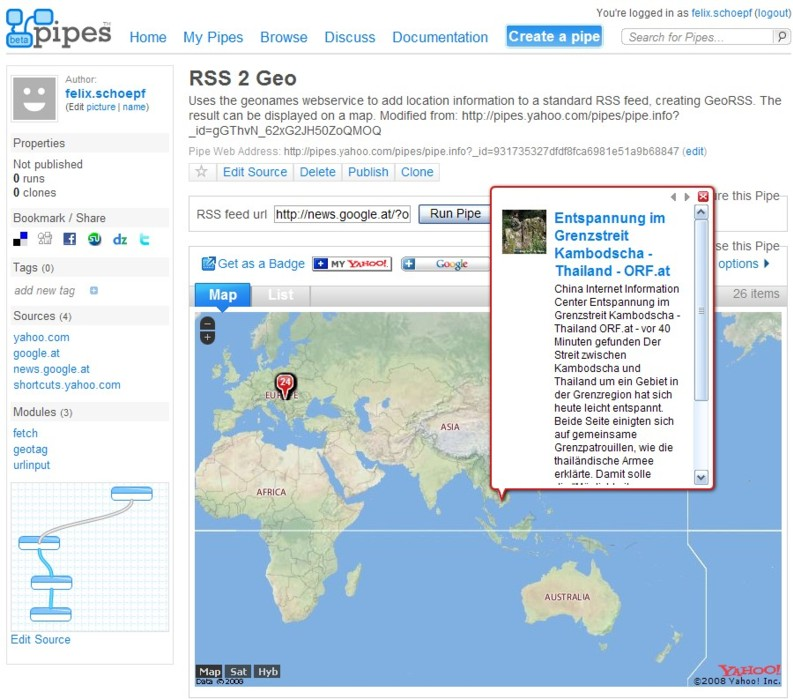
\includegraphics{Bilder/yahoo_pipes_google_news.jpg}}
	\caption{Yahoo Pipes - Running a pipe}
	\label{fig:yahoo_pipes_google_news}
\end{figure}

\begin{figure}
	\centering
		\fbox{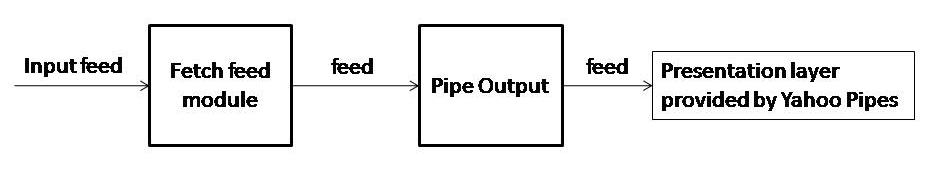
\includegraphics[width=0.8\textwidth]{Bilder/yahoo_pipes_simple_mashup.jpg}}
	\caption{Yahoo Pipes - Simple Mashup}
	\label{fig:yahoo_pipes_simple_mashup}
\end{figure}

\begin{figure}
	\centering
		\fbox{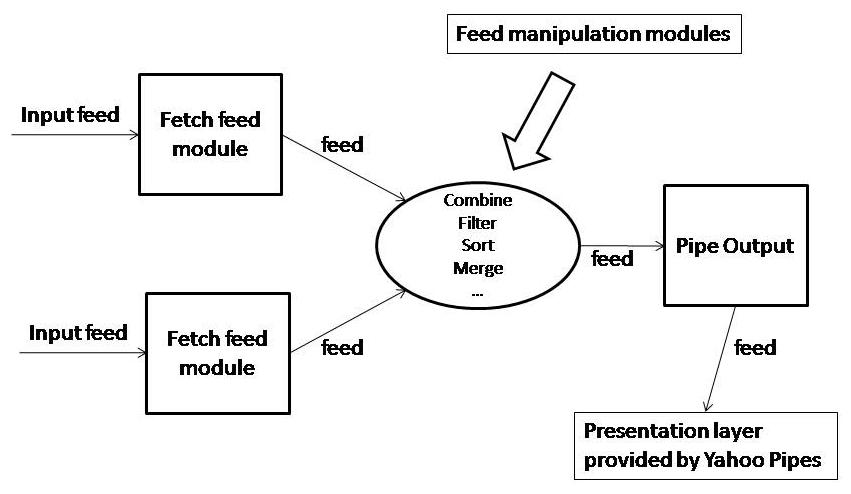
\includegraphics[width=0.8\textwidth]{Bilder/yahoo_pipes_complex_mashup.jpg}}
	\caption{Yahoo Pipes - Complex Mashup}
	\label{fig:yahoo_pipes_complex_mashup}
\end{figure}

\paragraph{Mashup Execution}
Similar to Microsoft, Yahoo makes a difference between build and runtime. As soon as a pipe is
``run'' a new browser window or tab opens and displays the output. Switching between the build and
runtime windows allows a quick adaptation of the current pipe.

\paragraph{Using the created Pipe}
Finally, if the development process is finished and the intended goals are
reached the pipe can be saved, published to other Yahoo Pipes users, to the
private Yahoo or Google page or to various social networking sites and
integrated into a website or a blog.

\subsubsection{IBM Mashup Center}
\label{sec:ibm_mashup_center}

Finally, the third tool to be tested is the ``IBM Mashup Center''
\cite{ibm_mashup_center}, which is focused on enterprise customers and
therefore resulted in a more complex application.

The Mashup Center mainly consists of two separate software products: ``InfoSphere MashupHub'' and ``Lotus
Mashups''. InfoSphere MashupHub is used for preparing all data sources and Louts Mashups is the
tool for composing the actual mashup (see Figure \ref{fig:ibm_mashup_center_concept}).

\begin{figure}
	\centering
		\fbox{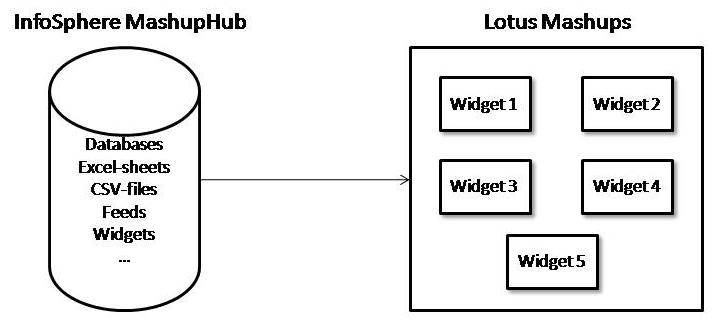
\includegraphics[width=0.8\textwidth]{Bilder/ibm_mashup_center_concept.jpg}}
	\caption{IBM Mashup Center - Concept}
	\label{fig:ibm_mashup_center_concept}
\end{figure}

\paragraph{InfoSphere MashupHub}
InfoSphere MashupHub is a lightweight information management environment where data sources
like databases, external web sources, Excel- or CSV-sheets are installed (see Figure
\ref{fig:ibm_mashup_center_mashuphub_all}). Visual tools for creating, storing, transforming and
remixing data easily and quickly can be included in the MashupHub \cite{ibm_mashup_center}.\newline
This means that data does not have to be refined within Lotus Mashups and the mashup composition
process respectively. This is a point where IBM Mashup Center differs from Microsoft Popfly and Yahoo
Pipes, where also the blocks for refining and editing the given data have to be placed on the working
area of the composition tool, which obviously limits the space for composing the actual mashup.

As soon as all necessary data sources are prepared within InfoSphere MashupHub
(see Figure \ref{fig:ibm_mashup_center_mashuphub_all}) they can be explicitly
added to Lotus Mashups to be available during the mashup composition process.

\begin{figure}
	\centering
		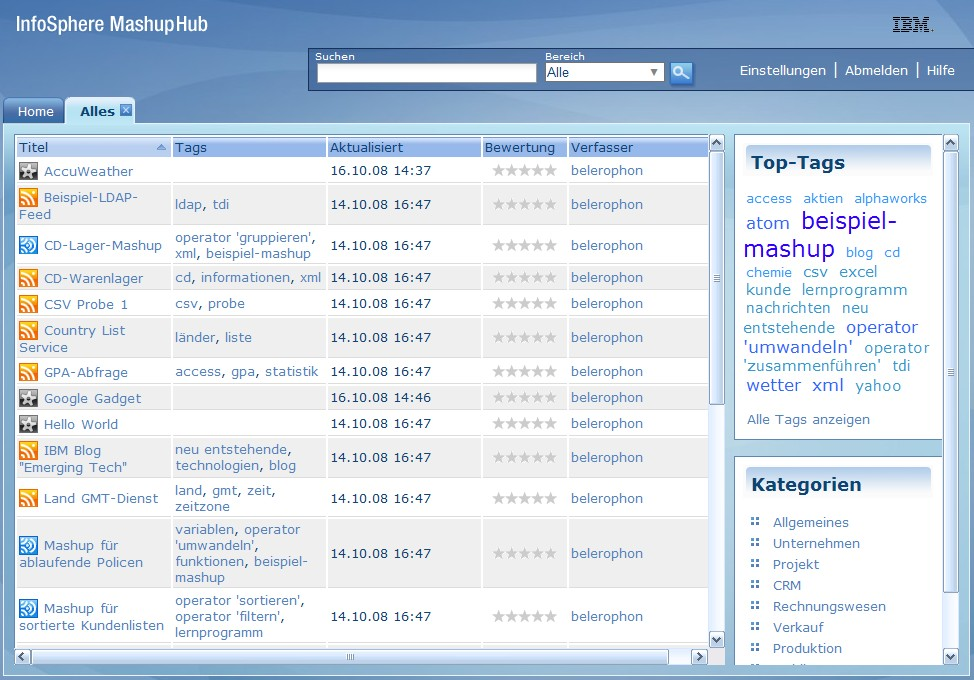
\includegraphics{Bilder/ibm_mashup_center_mashuphub_all.jpg}
	\caption{InfoSphere MashupHub - The Feeds, Widgets and Mashups}
	\label{fig:ibm_mashup_center_mashuphub_all}
\end{figure}

\paragraph{Lotus Mashups}
Lotus Mashups can have one or multiple sites, which are arranged in tabs. Furthermore, each site
provides a working area, where the building blocks can be placed on, has a name, can be deleted at
any time or made available for all other users of Lotus Mashups.

An additional search field can be used for finding components and data sources
respectively within InfoSphere MashupHub and thus adding them to the list of
available building blocks of Lotus Mashups.

\paragraph{The concept of a Mashup within IBM Mashup Center}
The base concept of Lotus Mashups are sites, where the widgets which display data can be arranged
(see Figure \ref{fig:ibm_mashup_center_mashups}). This means that the Mashup Center is more focused
on grouping widgets within sites and enabling data to be displayed in various forms on various sites
compared to the two other mashup composers.

Another big difference to Microsoft Popfly and Yahoo Pipes is the fact that
most mashups which were developed with these tools consist of only a single
widget within Lotus Mashups. This comes from the possibility of processing
data within Lotus Mashups and exposing the resulting data stream as widget.

But Lotus Mashups still provides the functionality to connect widgets, which
leads to the same structure than the other tools. Hence, a mashup consists of one or multiple
data source widgets, one or multiple data display widgets and connections between
them. Figure \ref{fig:ibm_mashup_center_mashups} depicts such a mashup: It
shows a data source widget, which displays customer data in a simple table and
is connected to three other widgets. One widget displays weather information
for the customers' address, another one displays the address on a map and the
third one shows the appropriate website.

Figure \ref{fig:ibm_mashup_center_mashup_concept} finally depicts the concept
behind such a mashup.

\begin{figure}
	\centering
		\fbox{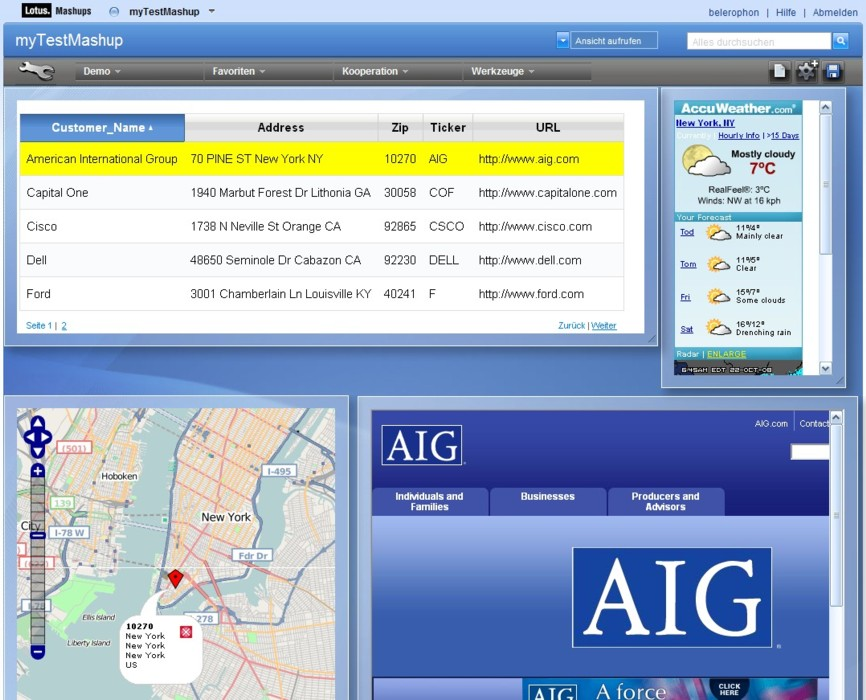
\includegraphics[width=0.8\textwidth]{Bilder/ibm_mashup_center_mashups.jpg}}
	\caption{Lotus Mashups - A sample Mashup}
	\label{fig:ibm_mashup_center_mashups}
\end{figure}


\begin{figure}
	\centering
		\fbox{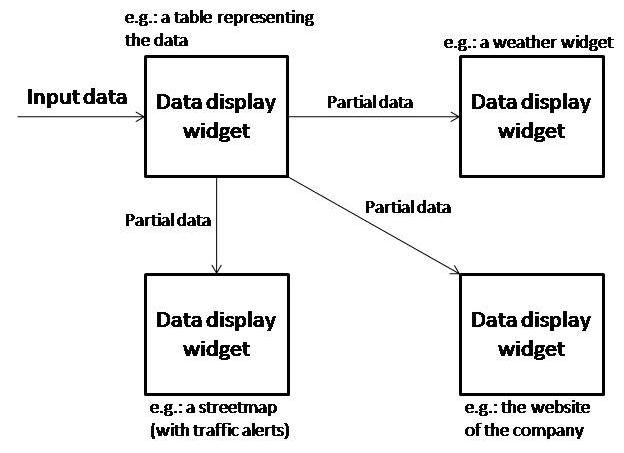
\includegraphics[width=0.7\textwidth]{Bilder/ibm_mashup_center_mashup_concept.jpg}}
	\caption{IBM Mashup Center - Mashup Concept}
	\label{fig:ibm_mashup_center_mashup_concept}
\end{figure}

\subsection{Evaluation Goal}

The goal of this evaluation is to obtain an impression of how powerful these mashup composers
are and how easy it is to develop small, but useful applications with them. Furthermore, the
evaluation should detect problems, which have to be solved, and missing features, which are
required to realize the discussed scenario (see Section \ref{sec:scenario}). Therefore, the next section introduces the
selected evaluation criteria.

\subsection{Evaluation Criteria}
\label{sec:evaluation_criterions}

\begin{itemize}
	\item \textbf{User Interface and Usability}\newline
	This part of the evaluation takes a closer look at the design and construction of the user
	interface. The user interface should be tailored towards end-users without programming experience
	and provide intuitive functionality to get quickly started.
	\item \textbf{Data Access and Processing}\newline
	The main goal of mashups is the processing of data from various data sources and thereby
	producing output data which is of value for the mashup consumer. Hence, every mashup
	composer has to provide building blocks which enable the access of various different data sources
	and furthermore provide blocks to combine, merge and process the received data. From this it
	follows that each tool also has to provide the functionality of exchanging data between
	blocks.
	\item \textbf{Extensibility}\newline
	This criterion takes a closer look at the possibility to extend the mashup composer with custom
	blocks to add special functionality and to adapt the mashup to the users' personal interests.
	\item \textbf{Multiple Instances}\newline
	Every mashup composer should be able to run multiple instances of the same component within a
	single mashup. This functionality is important for data access blocks, to fetch multiple
	data streams of the same format as well as for data processing and display blocks which are
	responsible for monitoring some kind of information, like the status of multiple flights (cf.
	Section \ref{sec:scenario}).
	\item \textbf{Grouping of Blocks}\newline
	As soon as a mashup gets more complex and multiple different data sets have to be displayed, the
	space provided by a single browser window is often too small. Therefore, the mashup composer tool
	should provide the functionality to group building blocks on different sites, which can be
	switched quickly.\newline Furthermore, two data sets that consist of multiple building blocks --
	like the monitor of an airplane (see Section \ref{sec:scenario}) -- have often to be compared.
	Hence, the tool should provide a feature to visually group the building blocks of one data set on the working area, to alleviate
	the comparison and to make the difference between the data sets more obvious.
	\item \textbf{Reusability of Groups}\newline
	This criterion deals with the reusability of grouped building blocks. Once a group is designed it
	should be able to save and reuse it either within the same or a different mashup. That means
	that a monitoring group for a single airplane (see Section \ref{sec:scenario}) can be saved and
	reused for a second airplane, by simply adapting the data source. The various groups can then
	be placed either on the same site or on different ones according to the use case.
	\item \textbf{Hot Deployment and Life-cycle Management}\newline
	This criterion addresses examples where created applications or mashups respectively should be
	adapted quickly without the need to restart the entire application.\newline Imagine the example
	from Section \ref{sec:scenario}, where the manager wants to monitor a changing number of
	airplanes over time. At the moment, the inspected mashup composers aren't flexible enough to
	display multiple groups of blocks on a single user interface or to add and remove a group or a
	monitored airplane respectively at runtime. However, for examples like this, it is necessary to
	enable the hot deployment of components which monitor an additional airplane as well as the
	functionality to stop a component and dispose it from the display as soon as the flight is over,
	without having to stop the monitoring process of other airplanes. From this it follows that the
	implemented components also require a life-cycle management within the running application.
	\item \textbf{Event Management}\newline
	This evaluation criterion deals with the provided possibilities of informing
	other blocks about events that occurred, without sending big amounts of data.
	That means that all interested blocks can register as event handlers for each
	specific event and hence can react to it, by, for example, updating the data source or
	opening an information window.\newline This mechanism can reduce
	the amount of data that is transferred and the coupling between blocks.\newline In connection with
	the air ambulance example (see Section \ref{sec:scenario}) the event management enables
	the propagation of technical problems concerning the airplane, information of the closedown of the
	destination airport and all the other events that can occur.
	\item \textbf{Logging}\newline
	The last criterion deals with the logging mechanism, which is needed for the logging of errors,
	warnings and other useful information. The acquired data can be used to analyze problems which
	occurred during the mashup creation and execution process and to apply data mining methods, which
	enable, for example, the analysis of user behavior.
\end{itemize}

\subsection{Rating}

In order to provide an overall assessment the inspected tools have been rated. For this purpose,
every mashup composer is awarded for each evaluation criterion (see Table
\ref{tab:TheEvaluationCriterions}) by either a ``+'', for fulfilling the respective criterion, or a
``o'' for the implementation of a partial solution or a ``-'' if the inspected criterion is missing.

\begin{table*}[h]
	\centering
		\begin{tabular}{|l|}
			\hline
				\textbf{Evaluation Criteria}\\
				\hline\hline
				User Interface and Usability\\
				\hline
				Data Access and Processing\\
				\hline
				Extensibility\\
				\hline
				Multiple Instances\\
				\hline
				Grouping of Blocks\\
				\hline
				Reusability of Groups\\
				\hline
				Hot Deployment and Life-cycle Management\\
				\hline
				Event Management\\
				\hline
				Logging\\
			\hline
		\end{tabular}
	\caption{Evaluation Criteria}
	\label{tab:TheEvaluationCriterions}
\end{table*}

\section{The Evaluation}

This section deals with the evaluation of the introduced mashup composers against the selected
evaluation criteria.
 
\subsection{User Interface and Usability}

Usability and the ease of use is one of the main goals of mashups. To enable the creation of simple
mashups by end-users, a clearly arranged, well structured and easy to use user interface is
indispensable.

\subsubsection{Microsoft Popfly}

For this purpose Microsoft Popfly groups its user interface into three main parts: A list of
available building blocks, which are categorized depending on their usage, a working area and a
help section. In addition, there are menu bars to edit the HTML-code, which surrounds the mashup,
to run the mashup as well as to save and share it.\newline Simple drag and drop enables the placing
of building blocks on the working area and the connection of these blocks. An additional interface
enables the adaptation of the input and output parameters of each block, which is necessary to
make them communicate and exchange data correctly.

\subsubsection{Yahoo Pipes}

Yahoo Pipes offers a user interface that looks quite similar to the one of Microsoft Popfly and
mainly consists of a list of building blocks and a working area. Furthermore, it provides detailed
information about each building block and a debugger console. This console displays the output of
the building block which is selected on the working area and hence constitutes a useful feature for
complex mashups. Again drag and drop is the way of creating pipes and connecting the single
building blocks.\newline Additional menu bars and buttons offer possibilities to create a new pipe,
save the current one, edit the properties of the mashup or execute it.

\subsubsection{IBM Mashup Center}

As IBM Mashup Center consists of two tools (i.e., Lotus Mashups and InfoSphere MashupHub) and is
designed for building sites containing various kinds of widgets, it is structured a little
differently.\newline Lotus Mashups -- the tool for designing the site -- provides a list of widgets
and a working area. Additional buttons enable the saving of the site and to browse the so-called
catalog, which is nothing else than a connection to the InfoSphere MashupHub, which constitutes the
repository for all widgets that can be used within Lotus Mashups.\newline As drag and drop is the
standard instrument to enable an easy and intuitive handling of applications it is also applied
within Lotus Mashups and enables the arrangement of the different widgets. The connection of the
widgets is not implemented by drawing visible arrows between the widgets, as with the two other
tools, but by specifying the target or source widget in a drop-down-list, which is provided by every
widget.

\subsubsection{Conclusion}

To sum up, all evaluated tools offer a well structured user interface, which is
easy and quite intuitive to use and enables the creation of a simple mashup within minutes.

The evaluation of the User Interface and Usability criterion hence leads to a balanced
result (cf. Table \ref{tab:RatingUserInterfaceAndUsability}).

\begin{table*}[h]
	\centering
		\begin{tabular}{|c|c|c|}
			\hline
				\textbf{Microsoft Popfly} & \textbf{Yahoo Pipes} & \textbf{IBM Mashup Center}\\
				\hline\hline
				+ & + & +\\
			\hline
		\end{tabular}
	\caption{Rating - User Interface and Usability}
	\label{tab:RatingUserInterfaceAndUsability}
\end{table*}

\subsection{Data Access and Processing}
\label{sec:data_access_and_aggregation}

This section evaluates the possibility of accessing and processing data with mashup composer tools.

\subsubsection{Microsoft Popfly}
Microsoft Popfly can access many data sources as long as they are published in the form of RSS feeds
or provide the data as character separated values. Furthermore, the catalog contains blocks to access
the Flickr database of photos or to get information from social networks like Digg or
Facebook. However, Popfly is limited to access data that is available on the web via simple
messaging standards. Local databases or data containers like Excel sheets remain unaccessible as long
as no custom block is implemented that provides this features.

To enable data processing Popfly provides blocks to combine data streams and to filter and sort
them. Unfortunately, no appropriate possibility to convert data from one format to another is
provided. This leads to data incompatibilities and constrains the communication between
blocks.\newline This problem leads to a limited number of blocks which can interact as long as no
custom blocks are implemented, which do the necessary conversion.

\subsubsection{Yahoo Pipes}
As Yahoo Pipes is designed to process feed data, it can fetch all kinds of RSS or Atom feeds which
are available on the web. Furthermore, it can access data which is available in CSV, XML or JSON
format as well as Yahoo search results and data from the Google merchant center, which constitutes
a database for products. Unfortunately, Yahoo Pipes also lacks the possibility to access
local databases or data containers like Excel and it is limited to data sets which are available or
can be converted to the RSS format.

For the purpose of processing data, Yahoo Pipes provides effective support. The data which is
fetched by the various modules is transformed to a RSS feed which can then be combined with other
feeds, filtered, sorted or split. For special processing the data can be sent to an external web
service which implements the necessary data transformation operations, which are not available
within Yahoo Pipes yet.

\subsubsection{IBM Mashup Center}
IBM Mashup Center allows the access of web feeds as well as of databases, Excel sheets, Access data
files and web services and hence provides more extensive data access means than the other two mashup
composers.

In the context of data processing IBM has to deal with the same problems as the other evaluated
tools. The provided building blocks for combining, filtering, extracting and transforming data, are
applicable for most of the pre-built blocks, but still there exist incompatible target blocks.
Hence, the user must implement sophisticated data transformation blocks to enable the communication
between all pre-built and custom blocks.

\subsubsection{Conclusion}

As none of the tools can completely fulfill the ``Data Access and Processing'' criterion, but
provide partial solutions, they are all rated with ``o'' (cf. Table
\ref{tab:RatingDataAccessAndAggregation}). Furthermore, it is important to mention that there will
exist data incompatibilities and hence data processing errors or problems, as long as mashup
composers do not make any restrictions on the used data format. Another solution for this problem is
the possibility of extending the tools with custom data transformation blocks and therewith placing
the responsibility for making a required data format compatible on the end-user.

\begin{table*}[h]
	\centering
		\begin{tabular}{|c|c|c|}
			\hline
				 \textbf{Microsoft Popfly} & \textbf{Yahoo Pipes} & \textbf{IBM Mashup Center}\\
				\hline\hline
				o & o & o\\
			\hline
		\end{tabular}
	\caption{Rating - Data Access and Processing}
	\label{tab:RatingDataAccessAndAggregation}
\end{table*}

\subsection{Extensibility}

The possibility to extend the available catalog of building blocks with custom blocks is an
important feature for each of the inspected tools and hence is evaluated in this section.

To fulfill this criterion Microsoft Popfly provides two mechanisms to develop custom blocks. Either
an existing block is edited or a new block is implemented by using the Visual Web Developer 2008
Express Edition. Also IBM Mashup Center can be extended by using an available software product,
namely the IBM Lotus Widget Factory. Yahoo Pipes, unfortunately, does not provide any possibilities
to extend its catalog of building blocks.

Table \ref{tab:Extensibility} displays the evaluation result for the ``Extensibility'' criterion.

\begin{table*}[h]
	\centering
		\begin{tabular}{|c|c|c|}
			\hline
				\textbf{Microsoft Popfly} & \textbf{Yahoo Pipes} & \textbf{IBM Mashup Center}\\
				\hline\hline
				+ & - & +\\
			\hline
		\end{tabular}
	\caption{Rating - Extensibility}
	\label{tab:Extensibility}
\end{table*}

\subsection{Multiple Instances}
\label{sec:multiple_instances}

Every mashup composer should provide an infrastructure that enables the execution of multiple
instances of the same building block in parallel. This is also a very important requirement for the
air ambulance example (see Section \ref{sec:scenario}) which has to display multiple airplanes at
the same time. It would be very impractical to have to implement a custom block for each airplane.
Hence, it should be possible to add multiple identical ``airplane components'' at the same time and
adapt the information they hold, by providing, for example, the flight number.

This criterion is fully realized by IBM Mashup Center and only partially by Microsoft Popfly and
Yahoo Pipes. These two tools limit the possibility to use multiple components, which are responsible
for displaying data, at the same time. That means that data source and processing components, which
are responsible for fetching and aggregating or converting data are handled differently than
display components.

Table \ref{tab:RatingMultipleInstances} holds the result for the ``Multiple Instances'' criterion.

\begin{table*}[h]
	\centering
		\begin{tabular}{|c|c|c|}
			\hline
				\textbf{Microsoft Popfly} & \textbf{Yahoo Pipes} & \textbf{IBM Mashup Center}\\
				\hline\hline
				o & o & +\\
			\hline
		\end{tabular}
	\caption{Rating - Multiple Instances}
	\label{tab:RatingMultipleInstances}
\end{table*}

\subsection{Grouping of Blocks}

The ``Grouping of Blocks'' criterion is neither realized by Microsoft Popfly nor by Yahoo Pipes
and only partially by the IBM Mashup Center. Indeed, IBM provides the possibility to group blocks
and widgets respectively within so-called ``sites'', which can be switched easily, but lacks the
feature of grouping blocks within a single site.

Therefore, Yahoo Pipes and Microsoft Popfly are awarded with a ``-'' and IBM Mashup Center with a
``o'' (cf. Table \ref{tab:RatingGroupingOfBlocks}).

\begin{table*}[h]
	\centering
		\begin{tabular}{|c|c|c|}
			\hline
				 \textbf{Microsoft Popfly} & \textbf{Yahoo Pipes} & \textbf{IBM Mashup Center}\\
				\hline\hline
				- & - & o\\
			\hline
		\end{tabular}
	\caption{Rating - Grouping of Blocks}
	\label{tab:RatingGroupingOfBlocks}
\end{table*}

\subsection{Reusability of Groups / Hot Deployment and Life-cycle Management / Event Management /
Logging}

As Microsoft Popfly and Yahoo Pipes lack the functionality of grouping blocks they also cannot
provide a mechanism to reuse groups and hence cannot score in the context of the ``Reusability of
Groups'' criterion. Unfortunately, also IBM Mashup Center fails to support the possibility to reuse
the created ``sites'' within other mashups.

Furthermore, each of the three tools differentiates between development and execution time. Hence,
none of the mashup composers supports hot deployment of additional components or provides life-cycle
support for components or building blocks respectively.

Although each of the evaluated tools provides the possibility to directly connect multiple building
blocks and to send data via these channels, none of them enables the more lightweight
publish-subscribe event mechanism (see Section \ref{sec:communication}).\newline Naturally the
direct connections can be misused for sending events, but this does not change the fact that the direct connections were introduced to
exchange data sets and require a tighter coupling than the event mechanism, which exchanges only
small pieces of information.

Finally, the evaluated mashup composers also miss a logging mechanism, which hence leads to the
evaluation results which are listed in Section \ref{sec:overall_evaluation_results}.

\subsection{Overall Evaluation Results}
\label{sec:overall_evaluation_results}

Table \ref{tab:RatingsTableWithoutWeightingFactors} shows the overall evaluation results concerning
the ratings each mashup tool was awarded with.

\begin{table*}[h]
	\centering
		\begin{tabular}{|c|c|c|c|c|c|c|c|c|c|}
			\hline
				\textbf{Evaluation Object} & 
				\begin{sideways}\textbf{User Interface and Usability}\end{sideways} &
				\begin{sideways}\textbf{Data Access and Processing}\end{sideways} &
                \begin{sideways}\textbf{Extensibility}\end{sideways} &
                \begin{sideways}\textbf{Multiple Instances}\end{sideways} &
                \begin{sideways}\textbf{Grouping of Blocks}\end{sideways} &
                \begin{sideways}\textbf{Reusability of Groups}\end{sideways} &
                \begin{sideways}\textbf{Hot Deployment and Life-cycle Management}\end{sideways} &
				\begin{sideways}\textbf{Event Management}\end{sideways} &
                \begin{sideways}\textbf{Logging}\end{sideways}\\
                \hline Microsoft Popfly 	& + & o & + & o & - & - & - & - & -\\
                \hline Yahoo Pipes 			& + & o & - & o & - & - & - & - & -\\
                \hline IBM Mashup Center 	& + & o & + & + & o & - & - & - & -\\
			\hline
		\end{tabular}
	\caption{Overall Ratings}
	\label{tab:RatingsTableWithoutWeightingFactors}
\end{table*}